\documentclass[11pt,letterpaper]{article}

\usepackage[T1]{fontenc}
\usepackage[utf8]{inputenc}
\usepackage{lmodern}
\usepackage[margin=1in]{geometry}
\usepackage{microtype}
\usepackage{amsmath}
\usepackage{amssymb}
\usepackage{xcolor}
\usepackage{booktabs}
\usepackage{tabularx}
\usepackage{enumitem}
\usepackage{titlesec}
\usepackage{parskip}
\usepackage{tikz}
\usepackage{pgfplots}
\usepackage[font=small,labelfont=bf]{caption}
\usepackage[hidelinks]{hyperref}

\pgfplotsset{compat=1.18}
\usetikzlibrary{arrows.meta, positioning}

\definecolor{accent}{HTML}{3B6D11}
\definecolor{titledark}{HTML}{2C4A20}
\definecolor{muted}{HTML}{5F5E5A}
\definecolor{rulegray}{HTML}{C9C7BE}
\definecolor{rubisco}{HTML}{1D9E75}
\definecolor{rubp}{HTML}{7F77DD}
\definecolor{tpu}{HTML}{D85A30}
\definecolor{boxfill}{HTML}{F1EFE8}

\titleformat{\section}{\normalfont\large\bfseries\color{accent}}{}{0pt}{}
\titlespacing*{\section}{0pt}{1.4em}{0.5em}

\newcommand{\Vcmax}{\ensuremath{V_{\mathrm{cmax}}}}
\newcommand{\Jmax}{\ensuremath{J_{\mathrm{max}}}}
\newcommand{\Rd}{\ensuremath{R_{\mathrm{d}}}}
\newcommand{\Ci}{\ensuremath{C_{\mathrm{i}}}}
\newcommand{\Ca}{\ensuremath{C_{\mathrm{a}}}}
\newcommand{\Cc}{\ensuremath{C_{\mathrm{c}}}}
\newcommand{\Gs}{\ensuremath{\Gamma^{*}}}
\newcommand{\umol}{\ensuremath{\mu}mol}

% A recorded question, set off by a hairline rule.
\newcommand{\question}[1]{%
  \vspace{1.5em}%
  {\noindent\color{rulegray}\rule{\textwidth}{0.4pt}\par}%
  \vspace{0.7em}%
  {\noindent\color{accent}\bfseries #1\par}%
  \vspace{0.6em}%
}

\setlist[itemize]{leftmargin=1.4em, itemsep=0.35em, topsep=0.4em}

\tikzset{
  stage/.style={draw=rulegray, fill=boxfill, line width=0.4pt, rounded corners=2pt,
                text width=0.72\textwidth, inner sep=6pt, align=left},
  flow/.style={draw=muted, line width=0.5pt, -{Straight Barb[length=1.6mm]}},
}

\begin{document}

{\noindent\color{titledark}\LARGE\bfseries A--C\lowercase{i} curves\par}
\vspace{0.4em}
{\noindent\color{rulegray}\rule{\textwidth}{0.8pt}\par}
\vspace{0.5em}
{\noindent\color{muted}\itshape One gas-exchange measurement that reads out three
different bottlenecks, and everything you have to trust to believe it.\par}
\vspace{1.2em}

{\noindent\color{muted}\small Recorded as a question-and-answer session, 18--20
September 2026. Questions are Prabu's, lightly tidied for spelling; answers are
Claude's, condensed from the conversation.\par}

\question{Give me an accessible tutorial on the A--\Ci{} curve.}

Photosynthesis can be throttled by three different things, and which one binds
depends on how much CO$_2$ is available inside the leaf. So if you \emph{vary}
the CO$_2$ and watch assimilation respond, each bottleneck reveals itself in a
different part of the curve. One thirty-minute measurement, three parameters.

The model behind it --- Farquhar, von Caemmerer \& Berry (1980),
\href{https://doi.org/10.1007/BF00386231}{10.1007/BF00386231} --- says the leaf
achieves whichever potential rate is \emph{smallest}:

\begin{align*}
A_{\mathrm{c}} &= \Vcmax \frac{\Cc - \Gs}{\Cc + K_{\mathrm{c}}(1 + O/K_{\mathrm{o}})} - \Rd
   &&\text{Rubisco-limited}\\[0.2em]
A_{\mathrm{j}} &= J \frac{\Cc - \Gs}{4\Cc + 8\Gs} - \Rd
   &&\text{RuBP-regeneration-limited}\\[0.2em]
A_{\mathrm{p}} &\approx 3\,\mathrm{TPU} - \Rd
   &&\text{triose-phosphate-limited}\\[0.4em]
A &= \min(A_{\mathrm{c}},\, A_{\mathrm{j}},\, A_{\mathrm{p}})
\end{align*}

That $\min$ is why the measured curve has a knee: you are watching the
limitation hand off. Here \Gs{} is the CO$_2$ compensation point in the absence
of respiration, $K_{\mathrm{c}}$ and $K_{\mathrm{o}}$ are Rubisco's kinetic
constants, and $O$ is oxygen. At saturating light $J \approx \Jmax$.

\begin{figure}[htbp]
\centering
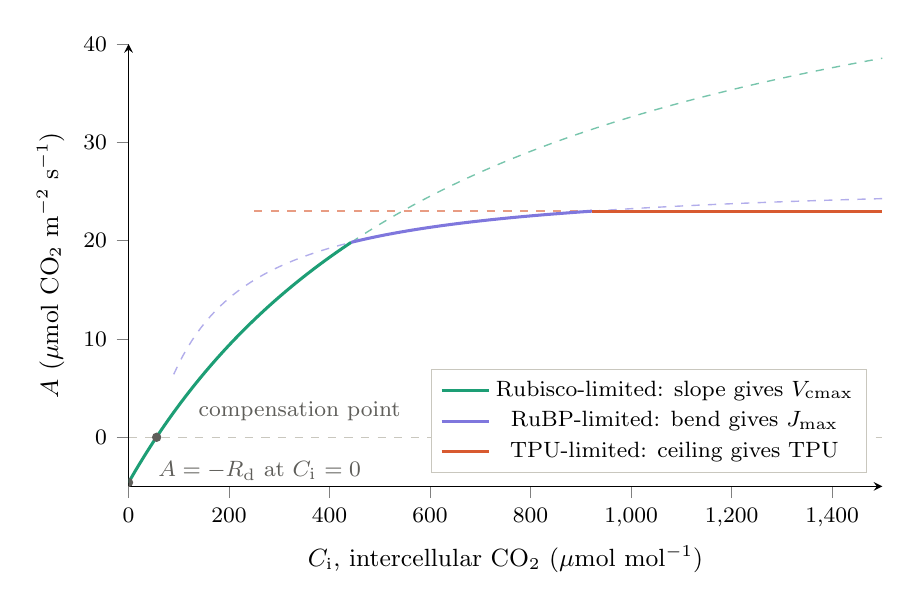
\begin{tikzpicture}
\begin{axis}[
  width=0.92\textwidth, height=7.2cm,
  xlabel={\Ci{}, intercellular CO$_2$ (\umol{} mol$^{-1}$)},
  ylabel={$A$ (\umol{} CO$_2$ m$^{-2}$ s$^{-1}$)},
  xmin=0, xmax=1500, ymin=-5, ymax=40,
  axis lines=left, tick align=outside,
  every axis plot/.append style={line width=1.1pt},
  label style={font=\small}, tick label style={font=\footnotesize},
  legend style={font=\footnotesize, draw=rulegray, at={(0.98,0.03)},
                anchor=south east, fill=white},
]
\addplot[dashed, rubisco, line width=0.5pt, opacity=0.6, domain=443:1500, samples=60, forget plot]
  {60*(x-42.75)/(x+710.3) - 1};
\addplot[dashed, rubp, line width=0.5pt, opacity=0.6, domain=90:443, samples=40, forget plot]
  {110*(x-42.75)/(4*x+342) - 1};
\addplot[dashed, rubp, line width=0.5pt, opacity=0.6, domain=922:1500, samples=20, forget plot]
  {110*(x-42.75)/(4*x+342) - 1};
\addplot[dashed, tpu, line width=0.5pt, opacity=0.6, domain=250:922, samples=2, forget plot] {23};

\addplot[rubisco, domain=0:443, samples=80] {60*(x-42.75)/(x+710.3) - 1};
\addlegendentry{Rubisco-limited: slope gives \Vcmax{}}
\addplot[rubp, domain=443:922, samples=40] {110*(x-42.75)/(4*x+342) - 1};
\addlegendentry{RuBP-limited: bend gives \Jmax{}}
\addplot[tpu, domain=922:1500, samples=2] {23};
\addlegendentry{TPU-limited: ceiling gives TPU}

\draw[rulegray, dashed, line width=0.4pt] (axis cs:0,0) -- (axis cs:1500,0);
\node[circle, fill=muted, inner sep=1.2pt] at (axis cs:0,-4.6) {};
\node[font=\footnotesize, color=muted, anchor=west] at (axis cs:40,-3.4)
  {$A = -\Rd$ at \Ci{} $=0$};
\node[circle, fill=muted, inner sep=1.2pt] at (axis cs:56,0) {};
\node[font=\footnotesize, color=muted, anchor=west] at (axis cs:120,2.6)
  {compensation point};
\end{axis}
\end{tikzpicture}
\caption{The measured curve (solid) is the lower envelope of three potential
rates. Dashed lines continue each potential rate into the region where it is not
limiting. Drawn from the Farquhar model with $\Vcmax = 60$, $\Jmax = 110$,
$\mathrm{TPU} = 8$, $\Rd = 1$.}
\label{fig:aci}
\end{figure}

\section{What you actually do at the bench}

Clamp a healthy, fully expanded, sun-exposed leaf into a gas-exchange chamber
--- LI-6800, LI-6400XT, Walz GFS-3000. Set saturating light (1500--2000 \umol{}
m$^{-2}$ s$^{-1}$ for a sun leaf), fix block temperature (25\,\textdegree C
conventionally) and keep VPD stable. Let it acclimate at ambient CO$_2$ until
$A$ and $g_{\mathrm{s}}$ stop drifting --- this can take 10--30 minutes and
people routinely rush it.

Then step the CO$_2$: down first, 400 $\to$ 300 $\to$ 200 $\to$ 150 $\to$ 100
$\to$ 50; back to 400 to let the stomata recover; then up, 600 $\to$ 800 $\to$
1000 $\to$ 1200 $\to$ 1500 (sometimes 2000). Two to three minutes per step,
logging once steady.

\textbf{Why down first?} High CO$_2$ closes stomata, and they reopen slowly. If
you went up first you would arrive at the low-CO$_2$ points with half-shut
stomata --- and those points are precisely the ones that determine \Vcmax{}.
Descending keeps the stomata open while you collect the part of the curve that
matters most.

\section{Reading the curve}

\begin{itemize}
  \item \textbf{Initial rise $\to$ \Vcmax{}.} CO$_2$ is scarce, Rubisco cannot
        grab it fast enough, so the slope reports how much active Rubisco is
        present.
  \item \textbf{The bend flattening out $\to$ \Jmax{}.} CO$_2$ is now plentiful
        and the limit becomes how fast electron transport regenerates RuBP.
  \item \textbf{The flat ceiling $\to$ TPU.} The Calvin cycle outruns the
        leaf's ability to turn triose phosphate into sucrose and starch;
        phosphate gets stranded and the whole thing caps out. Sometimes $A$
        declines slightly.
  \item \textbf{The intercept $\to$ \Rd{}.} Extrapolating to \Ci{} $=0$,
        assimilation is negative, and that offset is respiration. Measure
        $R_{\mathrm{dark}}$ directly in darkness if you care about it --- the
        extrapolated value is much less reliable.
\end{itemize}

\section{Fitting it}

Nearly everyone uses Sharkey et al. (2007),
\href{https://doi.org/10.1111/j.1365-3040.2007.01710.x}{10.1111/j.1365-3040.2007.01710.x},
and its spreadsheet, or the R package \texttt{plantecophys} --- Duursma (2015),
\href{https://doi.org/10.1371/journal.pone.0143346}{10.1371/journal.pone.0143346}
--- whose \texttt{fitaci()} does this in one call. Temperature normalisation to
25\,\textdegree C follows Bernacchi et al. (2001),
\href{https://doi.org/10.1111/j.1365-3040.2001.00668.x}{10.1111/j.1365-3040.2001.00668.x}.

The one genuinely subjective step is \textbf{assigning each point to a
limitation}. Automated fitters guess the breakpoints; different guesses give
different \Vcmax{}. Always plot the fit with the assignments shown.

\section{Where curves go wrong}

\begin{itemize}
  \item \textbf{Too few low-\Ci{} points.} You want at least four below \Ci{}
        $\approx 250$, or \Vcmax{} rests on almost nothing.
  \item \textbf{Not going high enough.} Stop at 1200 and you may never reach
        TPU --- and if TPU \emph{was} limiting your top points, it silently
        corrupts \Jmax{}.
  \item \textbf{Chamber leaks.} Gaskets leak when inside and outside CO$_2$
        differ sharply, which is exactly your endpoints. Run an empty-chamber
        correction.
  \item \textbf{Patchy stomatal closure.} Stressed leaves close in patches; the
        computed \Ci{} then describes no real part of the leaf.
  \item \textbf{\Ci{} versus \Cc{}.} The equations want CO$_2$ at Rubisco, but
        you measured it in the airspace. Ignoring mesophyll conductance
        typically underestimates \Vcmax{} by 20--30\,\% --- fine if you are
        consistent, a problem when comparing against studies that corrected
        for it.
\end{itemize}

\section{Sanity checks}

For C$_3$ leaves at 25\,\textdegree C: \Vcmax{} roughly 20--120 \umol{}
m$^{-2}$ s$^{-1}$ (crops at the high end, shade leaves low), \Jmax{} about
1.6--2$\times$ \Vcmax{}, \Rd{} around 0.5--2. In Figure~\ref{fig:aci} the TPU
ceiling sits at $3 \times 8 - 1 = 23$, which is where the curve goes flat. If
\Jmax{}:\Vcmax{} comes out at 4, or \Vcmax{} at 300, something went wrong in the
fit --- usually points assigned to the wrong limitation.

\question{``So if you vary the CO$_2$ and watch assimilation respond'' --- what
assimilation are you referring to?}

Net CO$_2$ assimilation rate, the $A$ on the $y$-axis: the rate at which a patch
of leaf removes CO$_2$ from the air.

Net, because the leaf is doing two opposing things at once. Photosynthesis
consumes CO$_2$; respiration and photorespiration release it. From outside you
can only see the balance:
\[
A \;=\; \text{gross photosynthesis} \;-\; \text{photorespiration} \;-\;
\text{mitochondrial respiration}
\]
Positive $A$ means the leaf is a net carbon sink. Negative --- in darkness, or
below the compensation point --- means net source. Gas exchange alone cannot
separate the components, which is why \Rd{} has to be measured in the dark, and
why $-\Rd$ appears explicitly in all three Farquhar equations: \Vcmax{}, \Jmax{}
and TPU describe \emph{gross} capacities, and you subtract respiration to get
what the instrument sees.

\question{Is \Ci{} the amount of CO$_2$ in the chamber?}

No --- that is \Ca{}. \Ci{} is the CO$_2$ \emph{inside} the leaf, in the air
spaces behind the stomata. There is a gradient, and CO$_2$ drops at every step:

\begin{center}
\begin{tabular}{@{}ll@{}}
\toprule
\Ca{} & chamber air --- you set this: 400, 300, 200 \ldots\\
\quad$\downarrow$ & stomata ($g_{\mathrm{s}}$)\\
\Ci{} & intercellular spaces --- calculated; the $x$-axis\\
\quad$\downarrow$ & mesophyll ($g_{\mathrm{m}}$)\\
\Cc{} & chloroplast stroma --- what Rubisco actually sees\\
\bottomrule
\end{tabular}
\end{center}

The curve is plotted against \Ci{} rather than \Ca{} because photosynthesis
responds to the CO$_2$ that reaches the leaf interior, not to what you dialled
into the chamber. Between the two sits stomatal conductance, which the leaf
controls and which varies during the measurement.

\Ci{} is never measured --- it is inferred. Diffusion through the stomata
follows Fick's law, so
\[
A = g_{\mathrm{s}}(\Ca - \Ci)
\qquad\Longrightarrow\qquad
\Ci = \Ca - A/g_{\mathrm{s}}.
\]
The instrument applies a fuller version that accounts for water vapour leaving
as CO$_2$ enters, but the principle holds: \Ci{} is a \emph{derived} quantity
resting on measured $A$ and $g_{\mathrm{s}}$.

Three practical consequences:

\begin{itemize}
  \item \Ci{} sits well below \Ca{}. In a healthy C$_3$ leaf at ambient,
        $\Ci/\Ca \approx 0.7$ --- set the chamber to 400 and \Ci{} lands near
        280.
  \item Evenly spaced setpoints produce unevenly spaced data. You stepped
        400\,$\to$\,300\,$\to$\,200, but \Ci{} moves by whatever the stomata
        allow.
  \item This is the weak link. Everything depends on $g_{\mathrm{s}}$ being
        right and uniform. With patchy stomatal closure, different parts of the
        leaf have genuinely different \Ci{}, and the single computed number
        describes none of them.
\end{itemize}

And the last step of the gradient is the one the standard fit ignores: $\Cc <
\Ci$, because CO$_2$ must still cross cell walls and membranes. Fitting against
\Ci{} when the equations want \Cc{} is exactly the 20--30\,\% \Vcmax{}
underestimate noted above.

\question{What is $g_{\mathrm{s}}$?}

Stomatal conductance --- how readily gas passes through the stomata, the
adjustable pores on the leaf surface. It is the inverse of a resistance: high
$g_{\mathrm{s}}$ means pores wide open and gas moving freely. Units are mol
m$^{-2}$ s$^{-1}$. A well-watered C$_3$ leaf runs about 0.1--0.6; a
water-stressed leaf can drop below 0.05.

It appears in the \Ci{} calculation because it sets how steep the CO$_2$
drawdown must be. For a given uptake $A$, narrow pores force a large gap between
outside and inside --- CO$_2$ has to be pulled far down to keep flowing through
a tight opening.

\textbf{It is measured through water, not CO$_2$.} The instrument computes
$g_{\mathrm{s}}$ from transpiration: it knows the humidity of air entering and
leaving, so it knows how much water vapour the leaf released, and it knows the
vapour-pressure gradient driving it. Conductance is flux over gradient. The
CO$_2$ conductance is that value divided by about 1.6. This is why leaf gas
exchange measures water and carbon at once, and why $A$ and $g_{\mathrm{s}}$
always arrive together in the data file.

$g_{\mathrm{s}}$ is under the plant's active control, responding to CO$_2$,
light, humidity and water status on a timescale of minutes --- that is, during
your measurement. Hence descending the CO$_2$ sequence first, and hence the fact
that every \Ci{} inherits the uncertainty in $g_{\mathrm{s}}$. It also gives the
intrinsic water-use efficiency, $A/g_{\mathrm{s}}$: carbon gained per unit of
stomatal opening.

\question{So the LI instrument measures and reports $g_{\mathrm{s}}$?}

It is a column in the output file, but computed, not sensed. The distinction
matters because it is where errors come from.

The instrument physically measures CO$_2$ and H$_2$O concentrations entering and
leaving the chamber, flow rate, leaf temperature, and chamber pressure.
Everything else is arithmetic on those. Transpiration comes from the humidity
difference and flow; conductance is then flux over driving gradient,
\[
E = g_{\mathrm{tw}}\,(w_{\mathrm{leaf}} - w_{\mathrm{air}}),
\]
where $w_{\mathrm{leaf}}$ is the saturation vapour concentration at leaf
temperature, assuming the internal air spaces are saturated. Invert for total
conductance, remove the boundary-layer term for stomatal conductance, divide by
${\approx}1.6$ for the CO$_2$ equivalent, and \Ci{} follows.

On an LI-6800 you see \texttt{gsw} alongside \texttt{gbw}, \texttt{gtw},
\texttt{gtc}, $A$, $E$ and \Ci{}; on the older LI-6400 the column is
\texttt{Cond}. A bare $g_{\mathrm{s}}$ in a paper means conductance to
\emph{water vapour} unless stated otherwise.

The chain of dependency is the point: $g_{\mathrm{s}}$ depends on leaf
temperature, \Ci{} depends on $g_{\mathrm{s}}$, \Vcmax{} depends on \Ci{}. Three
settings silently corrupt it, none of which the instrument can detect for you:

\begin{itemize}
  \item \textbf{Leaf area}, entered by hand. If the leaf does not fill the
        aperture and you leave the default, every flux is scaled wrong.
  \item \textbf{Stomatal ratio}, which sets the boundary-layer correction.
        Broadleaf trees are often hypostomatous, grasses amphistomatous.
  \item \textbf{Boundary-layer conductance} $g_{\mathrm{bw}}$, not measured per
        leaf but taken from a factory calibration for that chamber and fan
        speed.
\end{itemize}

\question{What is transpiration?}

Water evaporating out of the leaf --- the plant sweating through the same pores
it breathes through. Liquid water evaporates from wet cell surfaces inside the
leaf, saturating the internal air spaces; outside air is drier; that gradient
drives water vapour out through the stomata. In gas exchange it is $E$, in mmol
H$_2$O m$^{-2}$ s$^{-1}$ --- note \emph{milli}mol, against \umol{} for CO$_2$,
because the fluxes differ by roughly a thousandfold.

It is the unavoidable cost of photosynthesis. The leaf must open its stomata to
let CO$_2$ in, and the same opening lets water out, down a far steeper gradient.
A C$_3$ leaf typically loses on the order of hundreds of water molecules per
CO$_2$ fixed, which is why drought responses show up first as $g_{\mathrm{s}}$
closing.

For the measurement it does two jobs. First, it is how $g_{\mathrm{s}}$ gets
computed at all --- the instrument can see conductance only because water flows
through the same pores, driven by a gradient it can calculate. CO$_2$ cannot
serve that purpose, being consumed at an unknown rate; water is merely
diffusing. Second, it is the dilution correction: water vapour pouring out of
the leaf dilutes the air in the chamber, slightly lowering measured CO$_2$.
Ignore it and you would mis-attribute that dilution to photosynthetic uptake.

The driving force is the leaf-to-air vapour pressure deficit, which depends on
leaf temperature --- which is why thermocouple placement gets fussed over.

\question{Is $g_{\mathrm{s}}$ different for different gases?}

Yes. Same pore, different gas, different conductance: the geometry is identical,
what changes is how fast each molecule diffuses through air.

\textbf{Stomatal conductance: divide by 1.6.}
$g_{\mathrm{sc}} = g_{\mathrm{sw}}/1.6$. Water vapour diffuses faster than
CO$_2$, for a reason close to Graham's law --- lighter molecules move faster at
the same temperature, and $\sqrt{44/18} = 1.56 \approx 1.6$. Measured
diffusivities in air at 25\,\textdegree C agree: about $2.5 \times 10^{-5}$
m$^2$ s$^{-1}$ for water vapour against $1.6 \times 10^{-5}$ for CO$_2$.

\textbf{Boundary layer: divide by 1.37.}
$g_{\mathrm{bc}} = g_{\mathrm{bw}}/1.37$. The still air film at the leaf surface
is a second resistance in series, and transport across it is not pure molecular
diffusion --- it is partly stirred by airflow, so it scales with diffusivity to
the two-thirds power: $1.56^{2/3} \approx 1.37$. The two then combine per gas,
\[
1/g_{\mathrm{tc}} = 1/g_{\mathrm{sc}} + 1/g_{\mathrm{bc}},
\]
which is why the instrument reports \texttt{gsw}, \texttt{gbw}, \texttt{gtw} and
\texttt{gtc} as separate columns.

This extends even to isotopes of the same gas: $^{13}$CO$_2$ is slightly heavier
than $^{12}$CO$_2$ and diffuses about 4.4\,\textperthousand{} more slowly
through stomata. That discrimination is the mechanistic basis of leaf
$\delta^{13}$C as a water-use-efficiency proxy.

\question{What is the unit of $A$, and how is it calculated?}

\textbf{\umol{} CO$_2$ m$^{-2}$ s$^{-1}$} --- micromoles of CO$_2$ per square
metre of leaf area per second. Micromoles because the flux is tiny; per square
metre so the rate is comparable across leaves; per second because it is a rate.

The calculation is a mass balance on the air stream:
\[
A \;=\; \underbrace{\frac{F\,(C_{\mathrm{r}} - C_{\mathrm{s}})}{S}}_{\text{CO}_2\ \text{drawdown}}
   \;-\; \underbrace{C_{\mathrm{s}} \cdot E}_{\text{dilution correction}}
\]
with $F$ the flow rate through the chamber, $C_{\mathrm{r}}$ and
$C_{\mathrm{s}}$ the CO$_2$ entering and leaving, $S$ the enclosed leaf area
(typed in by hand), and $E$ transpiration.

The first term is the whole idea: air goes in at 400 ppm, comes out at 380, and
the 20\,ppm difference times the flow rate is CO$_2$ per second, divided by area
to make it a flux. The second term corrects for the fact that some of that drop
is dilution by transpired water rather than uptake.

\textbf{Worked example.} Flow 500 \umol{} s$^{-1}$, CO$_2$ falling from 400 to
380 \umol{} mol$^{-1}$, leaf area 6 cm$^2$:
\begin{align*}
(500 \times 10^{-6}\ \mathrm{mol\ s^{-1}}) \times (20 \times 10^{-6})
  &= 1 \times 10^{-8}\ \mathrm{mol\ CO_2\ s^{-1}} = 0.01\ \umol\ \mathrm{s^{-1}}\\
0.01\ \umol\ \mathrm{s^{-1}} \div 6 \times 10^{-4}\ \mathrm{m^2}
  &\approx 16.7\ \umol\ \mathrm{m^{-2}\ s^{-1}}
\end{align*}
Subtracting a dilution term of about 1.9 (see the next question) gives $A
\approx 14.8$ --- a healthy, well-lit C$_3$ leaf.

Three things that bite: leaf area is entered rather than measured, so a leaf
that does not fill the aperture scales every flux wrongly with nothing looking
suspicious; the drawdown must be resolvable, so flow rate has to be matched to
the expected $A$; and the two analysers must be matched, because you are taking
a small difference between two large numbers and any offset between them lands
directly in $A$.

\question{What is the unit of $E$ in that equation?}

In that equation $E$ must be in \textbf{mol H$_2$O m$^{-2}$ s$^{-1}$}, for the
units to close:
\[
C_{\mathrm{s}} \cdot E =
[\umol\ \mathrm{CO_2\ mol^{-1}\ air}] \times [\mathrm{mol\ H_2O\ m^{-2}\ s^{-1}}]
= \umol\ \mathrm{m^{-2}\ s^{-1}} \quad\checkmark
\]
which matches $A$. The term asks how much gas the leaf is adding to the stream,
so $E$ enters as a molar flux on the same basis as the air whose CO$_2$ fraction
$C_{\mathrm{s}}$ describes.

But it is \emph{reported} in mmol H$_2$O m$^{-2}$ s$^{-1}$ --- typical values
1--10, a more human-sized number. So when taking $E$ from a data file into this
equation, divide by 1000.

The sanity check is the size of the correction. With $E = 5$ mmol m$^{-2}$
s$^{-1}$ and $C_{\mathrm{s}} = 380$:
\begin{align*}
\text{correct:}\quad & 380 \times 0.005\ \mathrm{mol\ m^{-2}\ s^{-1}} = 1.9\ \umol\ \mathrm{m^{-2}\ s^{-1}} \quad (\approx 11\,\%\ \text{of}\ A)\\
\text{wrong:}\quad   & 380 \times 5\ \mathrm{mmol\ m^{-2}\ s^{-1}} = 1900\ \umol\ \mathrm{m^{-2}\ s^{-1}} \quad \text{(absurd)}
\end{align*}
A dilution correction of a few percent up to about 10\,\% is right. If yours
comes out comparable to $A$ itself, a factor of 1000 has slipped. Ignoring it
altogether overstates photosynthesis by more than a tenth, and the error grows
with transpiration --- largest on hot dry days with wide-open stomata, exactly
when stress responses are being measured.

\question{Remind me of the order of measured quantities and the inferred ones.}

Two groups, and the distinction matters.

\textbf{Genuinely sensed:} $C_{\mathrm{r}}$ and $C_{\mathrm{s}}$, the CO$_2$
entering and leaving, from the two infrared gas analysers; $W_{\mathrm{r}}$ and
$W_{\mathrm{s}}$, the same for water vapour; $F$, the flow rate;
$T_{\mathrm{leaf}}$, from a thermocouple or by energy balance; chamber air
temperature and pressure; and incident light.

\textbf{Not sensed at all:} leaf area $S$, the stomatal ratio, and the
boundary-layer conductance $g_{\mathrm{bw}}$ --- supplied by you, or by a
factory calibration for that chamber and fan speed.

Then the arithmetic, in strict order (LI-COR's unit conventions):
\begin{align*}
&\text{1.}\quad E = \frac{F\,(W_{\mathrm{s}} - W_{\mathrm{r}})}{S\,(1000 - W_{\mathrm{s}})}\\[0.3em]
&\text{2.}\quad w_{\mathrm{leaf}} = \text{saturation H$_2$O mole fraction at } T_{\mathrm{leaf}}
   \quad\longleftarrow\ T_{\mathrm{leaf}}\ \text{enters here}\\[0.3em]
&\text{3.}\quad g_{\mathrm{tw}} = \frac{E\,\bigl(1000 - (w_{\mathrm{leaf}} + W_{\mathrm{s}})/2\bigr)}{w_{\mathrm{leaf}} - W_{\mathrm{s}}},
   \qquad \frac{1}{g_{\mathrm{sw}}} = \frac{1}{g_{\mathrm{tw}}} - \frac{1}{g_{\mathrm{bw}}}\\[0.3em]
&\phantom{\text{3.}}\quad g_{\mathrm{sc}} = g_{\mathrm{sw}}/1.6,\quad
   g_{\mathrm{bc}} = g_{\mathrm{bw}}/1.37,\quad
   1/g_{\mathrm{tc}} = 1/g_{\mathrm{sc}} + 1/g_{\mathrm{bc}}\\[0.3em]
&\text{4.}\quad A = \frac{F\,(C_{\mathrm{r}} - C_{\mathrm{s}})}{S} - C_{\mathrm{s}} E\\[0.3em]
&\text{5.}\quad \Ci = \frac{(g_{\mathrm{tc}} - E/2)\,\Ca - A}{g_{\mathrm{tc}} + E/2}\\[0.3em]
&\text{6.}\quad \Vcmax,\ \Jmax,\ \mathrm{TPU},\ \Rd \ \longleftarrow\ \text{fitted to all the } (A, \Ci) \text{ pairs}
\end{align*}

\begin{figure}[htbp]
\centering
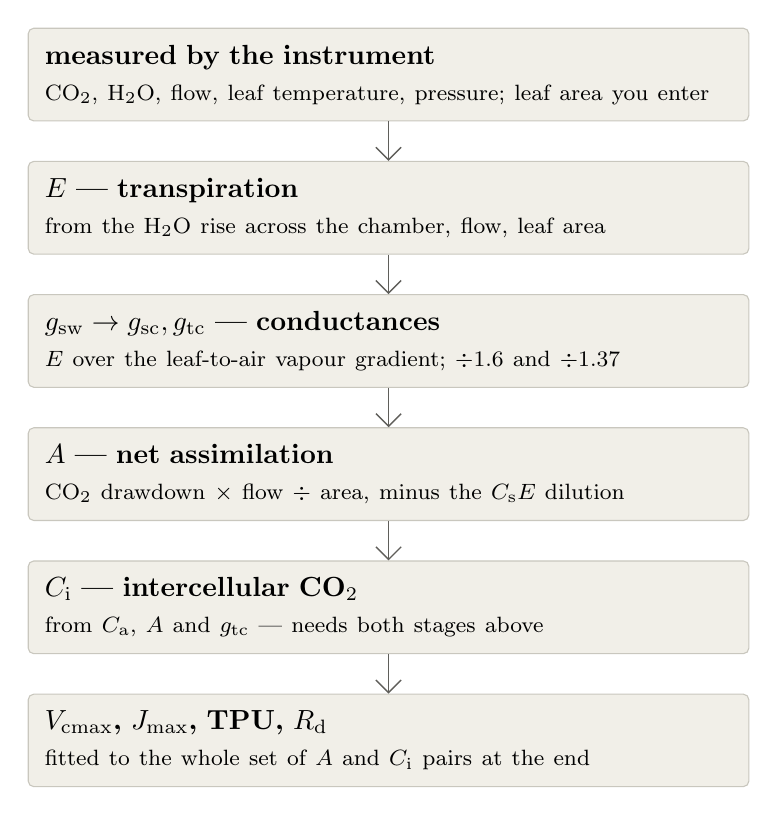
\begin{tikzpicture}[node distance=5mm]
\node[stage] (m) {\textbf{measured by the instrument}\\[1pt]
  {\footnotesize CO$_2$, H$_2$O, flow, leaf temperature, pressure; leaf area you enter}};
\node[stage, below=of m] (e) {\textbf{$E$ --- transpiration}\\[1pt]
  {\footnotesize from the H$_2$O rise across the chamber, flow, leaf area}};
\node[stage, below=of e] (g) {\textbf{$g_{\mathrm{sw}} \to g_{\mathrm{sc}}, g_{\mathrm{tc}}$ --- conductances}\\[1pt]
  {\footnotesize $E$ over the leaf-to-air vapour gradient; $\div 1.6$ and $\div 1.37$}};
\node[stage, below=of g] (a) {\textbf{$A$ --- net assimilation}\\[1pt]
  {\footnotesize CO$_2$ drawdown $\times$ flow $\div$ area, minus the $C_{\mathrm{s}}E$ dilution}};
\node[stage, below=of a] (c) {\textbf{\Ci{} --- intercellular CO$_2$}\\[1pt]
  {\footnotesize from \Ca{}, $A$ and $g_{\mathrm{tc}}$ --- needs both stages above}};
\node[stage, below=of c] (v) {\textbf{\Vcmax{}, \Jmax{}, TPU, \Rd{}}\\[1pt]
  {\footnotesize fitted to the whole set of $A$ and \Ci{} pairs at the end}};
\draw[flow] (m) -- (e);
\draw[flow] (e) -- (g);
\draw[flow] (g) -- (a);
\draw[flow] (a) -- (c);
\draw[flow] (c) -- (v);
\end{tikzpicture}
\caption{What the sensors see, and everything downstream that is arithmetic. An
error at any stage propagates to every stage below it.}
\label{fig:chain}
\end{figure}

Note what depends on what. $A$ needs only the CO$_2$ difference, the flow, the
area and $E$ --- it never touches $T_{\mathrm{leaf}}$. \Ci{} needs $A$
\emph{and} the whole conductance chain, so it inherits everything. Leaf
temperature enters at step 2, through the saturation vapour concentration, so
the real propagation path is
\[
T_{\mathrm{leaf}}\ \text{error} \;\to\; \mathrm{VPD}_{\mathrm{leaf}} \;\to\;
g_{\mathrm{tw}},\, g_{\mathrm{sw}} \;\to\; g_{\mathrm{tc}} \;\to\; \Ci \;\to\;
\Vcmax .
\]
$A$ and $E$ survive a bad thermocouple; \Ci{} and everything fitted from it do
not. A leaf-temperature problem shows up as a distorted $x$-axis, not a
distorted $y$-axis, and that is much harder to spot by eye.

\question{What is an IRGA?}

An infrared gas analyser --- the sensor that measures CO$_2$ and water vapour
concentration. It is the heart of the instrument; everything else is plumbing
around it.

CO$_2$ and H$_2$O are asymmetric molecules, so their bonds absorb infrared light
at characteristic wavelengths --- CO$_2$ strongly near 4.26 \textmu m, water
vapour near 2.6 \textmu m. Shine infrared through a tube of gas, measure how
much survives, and the absorption gives the concentration. Beer--Lambert,
essentially, with a single-wavelength detector rather than a spectrum.

There are two of them because the whole measurement is a \emph{difference}: a
reference analyser reads the air before the leaf, a sample analyser reads it
after. That difference might be 20\,ppm out of 400, so any mismatch between the
two lands straight in $A$. Hence \textbf{matching}: before a curve, the same air
is diverted to both analysers and their disagreement recorded and corrected. An
LI-6800 does this automatically at intervals. Skipping it is a classic way to
produce a beautiful-looking curve that is quietly wrong, and on an A--\Ci{}
curve the offset is not constant across the CO$_2$ range, so re-matching matters.

Leaf systems are \emph{open} --- air flows through continuously and you read the
steady-state difference. Closed systems seal a volume and watch concentration
fall over time. Open is better here because the leaf sits at a constant,
controlled CO$_2$ instead of a drifting one, which is exactly what you need when
CO$_2$ is the experimental variable.

\question{What is the difference between respiration and photorespiration?}

Both release CO$_2$, and that is where the resemblance ends.

\textbf{Respiration} is the standard cellular process --- the same one running
in your own cells. Sugars are broken down and oxidised, ultimately to CO$_2$ and
water, and the energy released is captured as ATP:
\[
\text{sugar} + \mathrm{O_2} \;\longrightarrow\; \mathrm{CO_2} + \mathrm{H_2O} + \text{ATP}
\]
Glycolysis in the cytosol, then the TCA cycle and oxidative phosphorylation in
the mitochondrion. Its purpose is to power the cell --- protein synthesis,
transport, growth, repair. Every living cell does it, in every tissue, day and
night. It is how a plant stays alive in darkness: the plant spending the carbon
it earned.

\textbf{Photorespiration} is a wasteful side reaction, and a consequence of one
enzyme's sloppiness. Rubisco cannot reliably distinguish CO$_2$ from O$_2$ ---
its full name is ribulose-1,5-bisphosphate carboxylase/\emph{oxygenase}, and
that second half is the problem. Roughly a quarter of the time in an ordinary
C$_3$ leaf, it attaches O$_2$ instead of CO$_2$. The product,
2-phosphoglycolate, is a two-carbon compound the plant cannot use and which
inhibits other enzymes if it accumulates. A salvage pathway recovers what it
can, running across chloroplast, peroxisome and mitochondrion, and in the
process releases CO$_2$ and burns ATP and reducing power. About three-quarters
of the carbon is recovered; the rest is lost. Nothing is gained --- it is damage
control.

\begin{center}
\small
\begin{tabularx}{\textwidth}{@{}lXX@{}}
\toprule
& \textbf{Respiration} & \textbf{Photorespiration}\\
\midrule
Purpose & produces usable energy & recovers from an enzymatic error\\
Net value & essential & a loss, ${\sim}25\,\%$ of potential photosynthesis in C$_3$ at moderate temperature\\
When & continuously, day and night & only in light, only while photosynthesis runs\\
Where & mitochondrion (plus cytosol) & chloroplast + peroxisome + mitochondrion\\
Consumes & sugars, O$_2$ & RuBP, O$_2$, ATP\\
Produces & CO$_2$, ATP & CO$_2$, and no usable energy\\
Occurs in & all organisms & only photosynthetic organisms\\
Suppressed by high CO$_2$ & no & yes\\
\bottomrule
\end{tabularx}
\end{center}

\textbf{Why photorespiration exists at all.} Rubisco evolved roughly three
billion years ago, in an atmosphere rich in CO$_2$ and nearly devoid of O$_2$.
Confusing the two molecules cost nothing then. Photosynthesis itself later
filled the air with oxygen, so the enzyme's flaw is a consequence of its own
success, and it has been stuck with it ever since. Evolution has improved
Rubisco's selectivity only marginally, apparently because greater specificity
comes at the price of a slower reaction. Some plants route around it rather than
fixing the enzyme: C$_4$ plants (maize, sugarcane) and CAM plants (cacti,
pineapple) concentrate CO$_2$ around Rubisco so that oxygenation rarely happens
--- an advantage that grows in hot, dry, bright conditions, which is where those
lineages dominate.

\textbf{Where each appears in the equations above.} Respiration is the explicit
$-\Rd$ term. Photorespiration has no term of its own --- it is hidden inside
\Gs{}, the CO$_2$ concentration at which carboxylation exactly balances the
CO$_2$ that photorespiration gives back, about 42.75 \umol{} mol$^{-1}$ at
25\,\textdegree C. The factor $(\Cc - \Gs)$ says only carbon fixed above that
break-even point counts, and the $4\Cc + 8\Gs$ denominator in
$A_{\mathrm{j}}$ encodes photorespiration's extra electron cost. So \Gs{} is the
\emph{photorespiratory} compensation point, while the point where the measured
curve crosses zero sits higher because it must also cover \Rd{}: in
Figure~\ref{fig:aci}, \Gs{} $\approx 43$ and the plotted compensation point
$\approx 56$, the gap between them being respiration.

\vspace{2em}
{\noindent\color{rulegray}\rule{\textwidth}{0.4pt}\par}
\vspace{0.5em}
{\noindent\color{muted}\small\itshape Sources checked against Crossref: Farquhar,
von Caemmerer \& Berry (1980); Sharkey et al.\ (2007); Bernacchi et al.\ (2001);
Duursma (2015). Instrument details refer to LI-COR LI-6400/LI-6800 conventions.\par}

\end{document}
